\documentclass[]{article}

%opening
\title{Exercises Set: Principal Components Analysis}
\author{DSBA Mathematics Refresher 2024}
\date{}

\usepackage{amsmath}
\usepackage{amsfonts}
\usepackage{amsthm}
\usepackage{amssymb}
\usepackage{mathrsfs}
\usepackage{stmaryrd}
\usepackage{graphicx}

\newcommand{\Q}{\mathbb{Q}}
\newcommand{\N}{\mathbb{N}}
\newcommand{\Z}{\mathbb{Z}}
\newcommand{\R}{\mathbb{R}}
\newcommand{\Primes}{\mathbb{P}}
\newcommand{\st}{\text{ s.t. }}
\newcommand{\txtand}{\text{ and }}
\newcommand{\txtor}{\text{ or }}
\newcommand{\lxor}{\veebar}


\begin{document}
	
	\maketitle
	
	\begin{abstract}
		Only the questions with a * are compulsory (but do all of them!).
	\end{abstract}	
	
	\section{Change of Basis}

	Let $\mathcal{B} = \{ \mathbf{e}_1, \mathbf{e}_2, \mathbf{e}_3 \}$ be the standard canonical basis for $\mathbb{R}^3$.

	Suppose we have another basis $\mathcal{B}' = \{ \mathbf{u}_1, \mathbf{u}_2, \mathbf{u}_3 \}$ for $\mathbb{R}^3$ and let $Q$ be the matrix whose columns are the coordinates of 
	$$
	\mathbf{u}_1 = \begin{pmatrix} 0.5 \\ -1 \\ 1 \end{pmatrix}_{\mathcal{B}}
	\textit{, }
	\mathbf{u}_2 = \begin{pmatrix} 2 \\ 0 \\ -1 \end{pmatrix}_{\mathcal{B}}
	\text{, and }
	\mathbf{u}_3 = \begin{pmatrix} -0.25 \\ 0.5 \\ 0 \end{pmatrix}_{\mathcal{B}}
	$$
	with respect to the standard basis.
	That is, $
	Q = \begin{bmatrix}
		\mathbf{u}_1 & \mathbf{u}_2 & \mathbf{u}_3
	\end{bmatrix}
	$.
	
	Let $\mathbf{v} = \begin{pmatrix} -1 \\ 3 \\ 2 \end{pmatrix}_{\mathcal{B}'}$.
	Express $\mathbf{v}$ in the standard basis $\mathcal{B}$.
	
	Let $\mathbf{w} = \begin{pmatrix} -1 \\ 3 \\ 2 \end{pmatrix}_{\mathcal{B}}$.
	Express $\mathbf{w}$ in the basis $\mathcal{B}'$.
	
	\section{Variance and Covariance}
	Calculate the variance of the following set:
	$$
	\mathcal{S}_1 = \{ 1.5, 3, 5, 7.5, 8, 9 \}
	$$
	Calculate the variance of the following set:
	$$
	\mathcal{S}_2 = \{ 0, 2, 4, 6, 8, 10 \}
	$$
	Calculate the covariance of $\mathcal{S}_1$ and $\mathcal{S}_2$.
	
	Compute $\hat{\mathcal{S}_1}$ and $\hat{\mathcal{S}_2}$, the standardized version of $\mathcal{S}_1$ and $\mathcal{S}_2$ (shifted to mean $0$ and scaled to have a variance of $1$).
	
	Calculate the covariance of $\hat{\mathcal{S}_1}$ and $\hat{\mathcal{S}_2}$. What do you remark?

	\section{Principal Component Analysis}
	Let $\mathcal{S} = \{ A, B, C, D, E, F \}$ be a set of $5$ points in $\mathbb{R}^3$.\\
	$A = \begin{pmatrix} 2 \\ -0.4 \\ 0.1 \end{pmatrix}$,
	$B = \begin{pmatrix} 4 \\ -0.8 \\ -0.1 \end{pmatrix}$,
	$C = \begin{pmatrix} 12 \\ -2.4 \\ -0.5 \end{pmatrix}$,
	$D = \begin{pmatrix} 12 \\ -2.4 \\ 0.5 \end{pmatrix}$,
	$E = \begin{pmatrix} 14 \\ -2.8 \\ -0.1 \end{pmatrix}$,\\
	and $F = \begin{pmatrix} 16 \\ -3.2 \\ 0.1 \end{pmatrix}$.
	
	\begin{center}
		\vspace{0.2cm}
		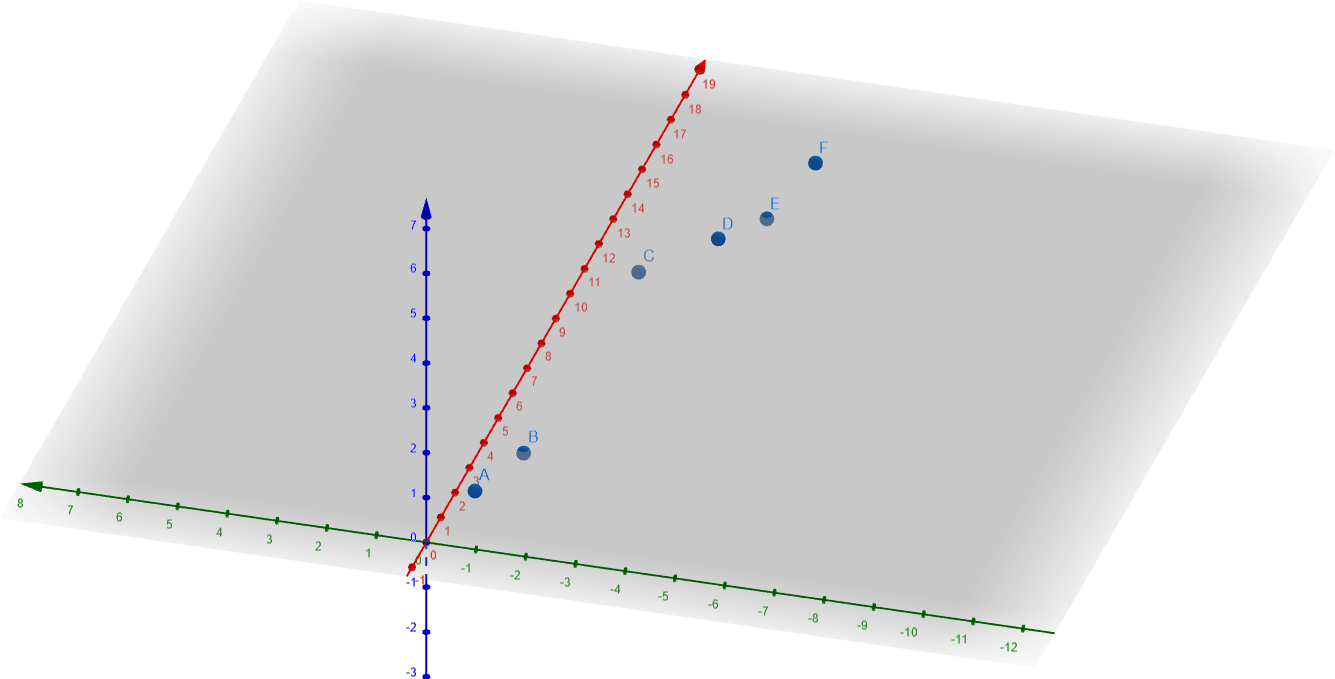
\includegraphics[width=0.95\linewidth]{points}
		\vspace{0.2cm}
	\end{center}
	
	\subsection{Standardization *}
	Calculate $\hat{\mathcal{S}}$, the standardized version of $\mathcal{S}$ (shifted to mean $0$ and scaled to have a variance of $1$).
	
	\subsection{Covariance matrix *}
	Compute the covariance of each pair of features.
	Compute also the variance of each feature.
	Arrange the values in a $3 \times 3$ matrix (variance is covariance of a feature with itself).
	
	\subsection{Eigenvalues of the covariance matrix *}
	Calculate the eigenvalues of the covariance matrix.
	Use the characteristic polynomial.
	
	The variance explained by each feature is $\frac{\lambda_i}{\lambda_1+\lambda_2+\lambda_3}$\footnote{Where $\lambda_i$ are the eigenvalues.}.
	Order the features by decreasing importance.
	
	\subsection{Feature vectors (the "principal components") *}
	For each eigenvalue, calculate the corresponding eigenvectors of the covariance matrix.
	These are the principal components, also called "feature vectors".
	
	\subsection{Recasting data on principal components axes *}
	Project each item of data on the first two components, and plot them in a 2D graph.
	
	\subsection{Importance of standardization}
	Redo this exercise without standardizing your data to variance of one.
	
	\section{Principal Component Analysis with Python}
	\textit{(see notebook)}
	
	\begin{center}
		\vspace{0.2cm}
		
\includegraphics[width=0.5\linewidth]{python}
		\vspace{0.2cm}
	\end{center}

\end{document}
